\documentclass{beamer}
\usepackage[utf8]{inputenc}

\usetheme{Madrid}
\usecolortheme{default}
\usepackage{amsmath,amssymb,amsfonts,amsthm}
\usepackage{mathtools}
\usepackage{txfonts}
\usepackage{tkz-euclide}
\usepackage{listings}
\usepackage{adjustbox}
\usepackage{array}
\usepackage{gensymb}
\usepackage{tabularx}
\usepackage{gvv}
\usepackage{lmodern}
\usepackage{circuitikz}
\usepackage{tikz}
\lstset{literate={·}{{$\cdot$}}1 {λ}{{$\lambda$}}1 {→}{{$\to$}}1}
\usepackage{multicol}
\usepackage{graphicx}

\setbeamertemplate{page number in head/foot}[totalframenumber]

\usepackage{tcolorbox}
\tcbuselibrary{minted,breakable,xparse,skins}



\definecolor{bg}{gray}{0.95}
\DeclareTCBListing{mintedbox}{O{}m!O{}}{%
  breakable=true,
  listing engine=minted,
  listing only,
  minted language=#2,
  minted style=default,
  minted options={%
    linenos,
    gobble=0,
    breaklines=true,
    breakafter=,,
    fontsize=\small,
    numbersep=8pt,
    #1},
  boxsep=0pt,
  left skip=0pt,
  right skip=0pt,
  left=25pt,
  right=0pt,
  top=3pt,
  bottom=3pt,
  arc=5pt,
  leftrule=0pt,
  rightrule=0pt,
  bottomrule=2pt,
  toprule=2pt,
  colback=bg,
  colframe=orange!70,
  enhanced,
  overlay={%
    \begin{tcbclipinterior}
    \fill[orange!20!white] (frame.south west) rectangle ([xshift=20pt]frame.north west);
    \end{tcbclipinterior}},
  #3,
}
\lstset{
    language=C,
    basicstyle=\ttfamily\small,
    keywordstyle=\color{blue},
    stringstyle=\color{orange},
    commentstyle=\color{green!60!black},
    numbers=left,
    numberstyle=\tiny\color{gray},
    breaklines=true,
    showstringspaces=false,
}
%------------------------------------------------------------
%This block of code defines the information to appear in the
%Title page
\title %optional
{12.560}
\date{September 20,2025}
%\subtitle{A short story}

\author % (optional)
{Harsha-EE25BTECH11026}



\begin{document}


\frame{\titlepage}


\begin{frame}{Question}
A scalar function is given by $f\brak{x,y}=x^2+y^2$. Take $\hat{i}$ and $\hat{j}$ as the unit vectors along the x and y axes, respectively. At $\brak{x,y}=\brak{3,4}$, the direction along which $f$ increases the fastest is
\begin{enumerate}
\begin{multicols}{4}
    \item $\frac{1}{5}\brak{4\hat{i}-3\hat{j}}$
    \item $\frac{1}{5}\brak{3\hat{i}-4\hat{j}}$
    \item $\frac{1}{5}\brak{3\hat{i}+4\hat{j}}$
    \item $\frac{1}{5}\brak{4\hat{i}+3\hat{j}}$
\end{multicols}
\end{enumerate}
\end{frame}

\begin{frame}{Theoretical Solution:Approach-1}
The direction vector along which the function $f\brak{x,y}$ is given by the gradient direction vector of the function, which is given by
\begin{align}
    \nabla f\brak{x,y}=\myvec{\tfrac{\partial f}{\partial x}\\\tfrac{\partial f}{\partial y}}
\end{align}
\begin{align}
    \therefore \nabla f\brak{x,y}=\myvec{2x\\2y}
\end{align}
At $\brak{x,y}=\brak{3,4}$,
\begin{align}
    \nabla f\brak{3,4}=\myvec{6\\8}
\end{align}
\begin{align}
    \implies \text{Direction vector: }\frac{1}{5}\myvec{3\\4}
\end{align}
\end{frame}


\begin{frame}[fragile]
    \frametitle{C Code -Finding displacement matrix}

    \begin{lstlisting}[language=C]
#include<stdio.h>

void dir_vec(double x, double y, double *grad){
	grad[0]=2*x;
	grad[1]=2*y;
}
    \end{lstlisting}
\end{frame}



\begin{frame}[fragile]
    \frametitle{Python+C code}

    \begin{lstlisting}[language=Python]
import sympy as sp
import numpy as np
import ctypes
import matplotlib.pyplot as plt

lib = ctypes.CDLL("./libmain.so")

lib.dir_vec.argtypes = (ctypes.c_double,ctypes.c_double,np.ctypeslib.ndpointer(dtype=np.float64, ndim=1, flags="C_CONTIGUOUS"))

px, py = 3, 4
grad = np.empty(2, dtype=np.float64)
lib.dir_vec(px, py, grad)


    \end{lstlisting}
\end{frame}

\begin{frame}[fragile]
    \frametitle{Python+C code}

    \begin{lstlisting}[language=Python]
norm_grad = np.linalg.norm(grad)
unit_grad = grad / norm_grad
unit_vec = sp.Matrix(unit_grad)
print("Unit vector along the direction of f:")
sp.pprint(unit_vec)

xx = np.linspace(-5, 5, 200)
yy = np.linspace(-5, 5, 200)
X, Y = np.meshgrid(xx, yy)
Z = X**2 + Y**2

plt.figure(figsize=(7,6))
contours = plt.contour(X, Y, Z, levels=20, cmap="viridis")
plt.clabel(contours, inline=True, fontsize=8)
    \end{lstlisting}
\end{frame}

\begin{frame}[fragile]
    \frametitle{Python+C code}

    \begin{lstlisting}[language=Python]
plt.scatter(px, py, color="red", label="Point (3,4)")

plt.quiver(px, py, grad[0], grad[1],angles="xy", scale_units="xy", scale=1, color="blue", width=0.005,label="Full ∇f at (3,4)")

plt.quiver(px, py, unit_grad[0], unit_grad[1],angles="xy", scale_units="xy", scale=1, color="green", width=0.005,label="Unit ∇f at (3,4)")
plt.xlabel("x-axis")
plt.ylabel("y-axis")
plt.title("Gradient and Unit Gradient at (3,4) for f(x,y) = x² + y²")
plt.legend()
plt.axis("equal")
plt.savefig("/home/user/Matrix Theory: workspace/Matgeo_assignments/12.560/figs/Figure_1.png")
plt.show()
    \end{lstlisting}
\end{frame}



\begin{frame}[fragile]
    \frametitle{Python code}
    \begin{lstlisting}[language=Python]
import sympy as sp
import matplotlib.pyplot as plt
import numpy as np

x, y = sp.symbols('x y')
f = x**2 + y**2

grad = sp.Matrix([sp.diff(f, v) for v in (x, y)])
px, py = 3, 4
grad_val = grad.subs({x: px, y: py})
norm_val = grad_val.norm()
unit_grad = grad_val / norm_val

print("Unit vector along the direction where f grows the fastest:")
sp.pprint(unit_grad)

grad_num = np.array([float(grad_val[0]), float(grad_val[1])])  
unit_grad_num = np.array([float(unit_grad[0]), float(unit_grad[1])])  
    \end{lstlisting}   
\end{frame}

\begin{frame}[fragile]
    \frametitle{Python code}
    \begin{lstlisting}[language=Python]
xx = np.linspace(-5, 5, 200)
yy = np.linspace(-5, 5, 200)
X, Y = np.meshgrid(xx, yy)
Z = X**2 + Y**2

plt.figure(figsize=(7,6))
contours = plt.contour(X, Y, Z, levels=20, cmap="viridis")
plt.clabel(contours, inline=True, fontsize=8)

plt.scatter(px, py, color="red", label="Point (3,4)")

plt.quiver(px, py, grad_num[0], grad_num[1], angles="xy", scale_units="xy", scale=1, color="blue", width=0.005,
label="Full ∇f at (3,4)")
    \end{lstlisting}   
\end{frame}

\begin{frame}[fragile]
    \frametitle{Python code}
    \begin{lstlisting}[language=Python]
# Draw unit gradient vector
plt.quiver(px, py, unit_grad_num[0], unit_grad_num[1], 
           angles="xy", scale_units="xy", scale=1, color="green", width=0.005,
           label="Unit ∇f at (3,4)")

plt.xlabel("x-axis")
plt.ylabel("y-axis")
plt.title("Gradient and Unit Gradient at (3,4) for f(x,y) = x² + y²")
plt.legend()
plt.axis("equal")
plt.savefig("/home/user/Matrix Theory: workspace/Matgeo_assignments/12.560/figs/Figure_1.png")
plt.show()
    \end{lstlisting}   
\end{frame}

\begin{frame}{Plot}
    \begin{figure}[H]
    \centering
    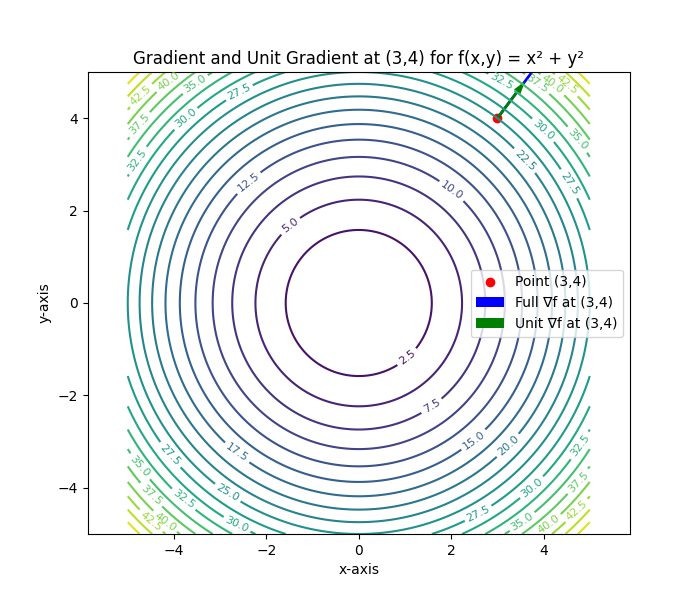
\includegraphics[width=0.8\columnwidth]{figs/Figure_1.png}
    \label{fig:1}
\end{figure}
\end{frame}

\begin{frame}{Theoretical Solution:Approach-2}
As the point is given to be $\myvec{3\\4}$, it can be assumed that for the circle,
\begin{align}
    \vec{x}^{\top}\vec{V}\vec{x}=3^2+4^2=25 \label{eq:1}
\end{align}
where $\vec{V}=\vec{I}$.\\
We can infer that the function will increse along the direction vector of normal at that point.
The direction vector of normal is given by
\begin{align}
    \vec{n}=\brak{\vec{V}\vec{q}+\vec{u}}
\end{align}
where, $\vec{q}$ is the point of contact.
\begin{align}
    \therefore \vec{n}=\myvec{1&&0\\0&&1}\myvec{3\\4}+\myvec{0\\0}=\myvec{3\\4}
\end{align}
\end{frame}


\begin{frame}[fragile]
    \frametitle{C Code -Finding displacement matrix}

    \begin{lstlisting}[language=C]
#include <stdio.h>

void normal_vector(double x, double y, double *result) {
    result[0] = x;
    result[1] = y;
}
    \end{lstlisting}
\end{frame}



\begin{frame}[fragile]
    \frametitle{Python+C code}

    \begin{lstlisting}[language=Python]
import ctypes
import sympy as sp
import matplotlib.pyplot as plt
import numpy as np

lib = ctypes.CDLL("./libnormal.so")

lib.normal_vector.argtypes = (ctypes.c_double, ctypes.c_double,
                              np.ctypeslib.ndpointer(dtype=np.float64, ndim=1, flags="C_CONTIGUOUS"))

x0, y0 = 3.0, 4.0
result = np.zeros(2, dtype=np.float64)
lib.normal_vector(x0, y0, result)
normal_vec = sp.Matrix(result)
print("Normal direction vector:")
sp.pprint(normal_vec)


    \end{lstlisting}
\end{frame}

\begin{frame}[fragile]
    \frametitle{Python+C code}

    \begin{lstlisting}[language=Python]
theta = np.linspace(0, 2*np.pi, 400)
circle_x = 5 * np.cos(theta)
circle_y = 5 * np.sin(theta)

plt.plot(circle_x, circle_y, label='Circle: x^2+y^2=25')
plt.plot(x0, y0, 'ro', label='Point (3,4)')
plt.quiver(x0, y0, result[0], result[1], angles='xy', scale_units='xy', scale=1,
           color='g', label='Normal vector')

plt.gca().set_aspect('equal', adjustable='box')
plt.axhline(0, color='k', linewidth=0.5)
plt.axvline(0, color='k', linewidth=0.5)
plt.legend()
plt.grid(True)
plt.savefig("/home/user/Matrix Theory: workspace/Matgeo_assignments/12.560/figs/Figure_2.png")
plt.show()
    \end{lstlisting}
\end{frame}

\begin{frame}[fragile]
    \frametitle{Python+C code}

    \begin{lstlisting}[language=Python]
plt.scatter(px, py, color="red", label="Point (3,4)")

plt.quiver(px, py, grad[0], grad[1],angles="xy", scale_units="xy", scale=1, color="blue", width=0.005,label="Full ∇f at (3,4)")

plt.quiver(px, py, unit_grad[0], unit_grad[1],angles="xy", scale_units="xy", scale=1, color="green", width=0.005,label="Unit ∇f at (3,4)")
plt.xlabel("x-axis")
plt.ylabel("y-axis")
plt.title("Gradient and Unit Gradient at (3,4) for f(x,y) = x² + y²")
plt.legend()
plt.axis("equal")
plt.savefig("/home/user/Matrix Theory: workspace/Matgeo_assignments/12.560/figs/Figure_1.png")
plt.show()
    \end{lstlisting}
\end{frame}



\begin{frame}[fragile]
    \frametitle{Python code}
    \begin{lstlisting}[language=Python]
import sympy as sp
import matplotlib.pyplot as plt
import numpy as np

x, y = sp.symbols('x y')
expr = x**2 + y**2 - 25

grad = sp.Matrix([sp.diff(expr, x), sp.diff(expr, y)])
q = {x: 3, y: 4}
normal_vec = grad.subs(q)
print("Normal direction vector:")
sp.pprint(normal_vec)  # pretty print as column vector 
    \end{lstlisting}   
\end{frame}

\begin{frame}[fragile]
    \frametitle{Python code}
    \begin{lstlisting}[language=Python]
# Circle parameters
theta = np.linspace(0, 2*np.pi, 400)
circle_x = 5 * np.cos(theta)
circle_y = 5 * np.sin(theta)
plt.plot(circle_x, circle_y, label='Circle: x^2+y^2=25')
plt.plot(3, 4, 'ro', label='Point (3,4)')

plt.quiver(3, 4, float(normal_vec[0]), float(normal_vec[1]),
           angles='xy', scale_units='xy', scale=1, color='g', label='Normal vector')

plt.gca().set_aspect('equal', adjustable='box')
plt.axhline(0, color='k', linewidth=0.5)
plt.axvline(0, color='k', linewidth=0.5)
plt.legend()
plt.grid(True)
plt.savefig("/home/user/Matrix Theory: workspace/Matgeo_assignments/12.560/figs/Figure_2.png")
plt.show()

    \end{lstlisting}   
\end{frame}


\begin{frame}{Plot}
    \begin{figure}[H]
    \centering
    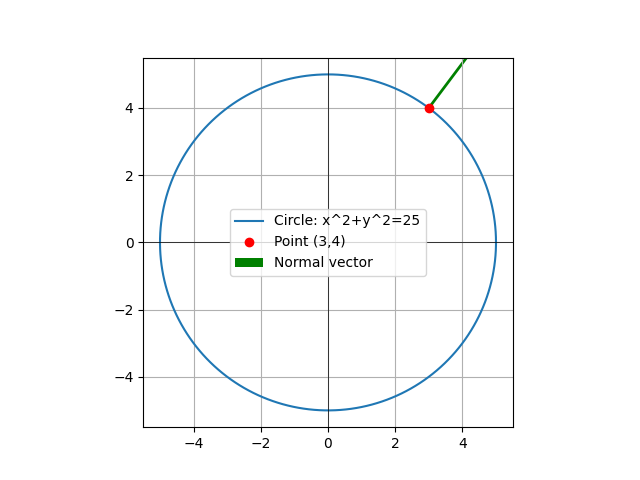
\includegraphics[width=0.7\columnwidth]{figs/Figure_2.png}
    \caption{Graph for approach-2}
    \label{fig:2}
    \end{figure}
\end{frame}



\end{document}